
\section{Функция последования. Точки отображения Пуанкаре}

	\begin{minipage}{0.4\textwidth}	
		$$
			\begin{cases}
	 			\dot{x} = f_1(x,y) \\
	 			\dot{y} = f_2(x,y)
			\end{cases} 
		$$
		Функция последования:
		$$
			\begin{gathered}
				\psi(a_0) = a_1 \\
				\psi(a_1) = a_2 \\ \cdots \\
				\psi(a_{k-1}) = a_k			
			\end{gathered}
		$$
		Отображение Пуанкаре:
		\newline
		$$
			\begin{gathered}
				\text{П} (a_0) = \psi(a_0) - \psi(a_1) \\ \cdots \\
				\text{П} (a_{k-1}) = \psi(a_{k-1}) - \psi(a_k) \\ 	
			\end{gathered}
		$$ 
	
	    \begin{center}
				\Big| $\psi$ определена, если поле \Big| \newline не меняет знак
		\end{center}
	\end{minipage}
	\hfill
	\begin{minipage}{0.6\textwidth}
		Пусть $\gamma$ --- такая кривая, которая \newline 
		\underline{не касается} траекторий (может пересекать)	
		\begin{center} 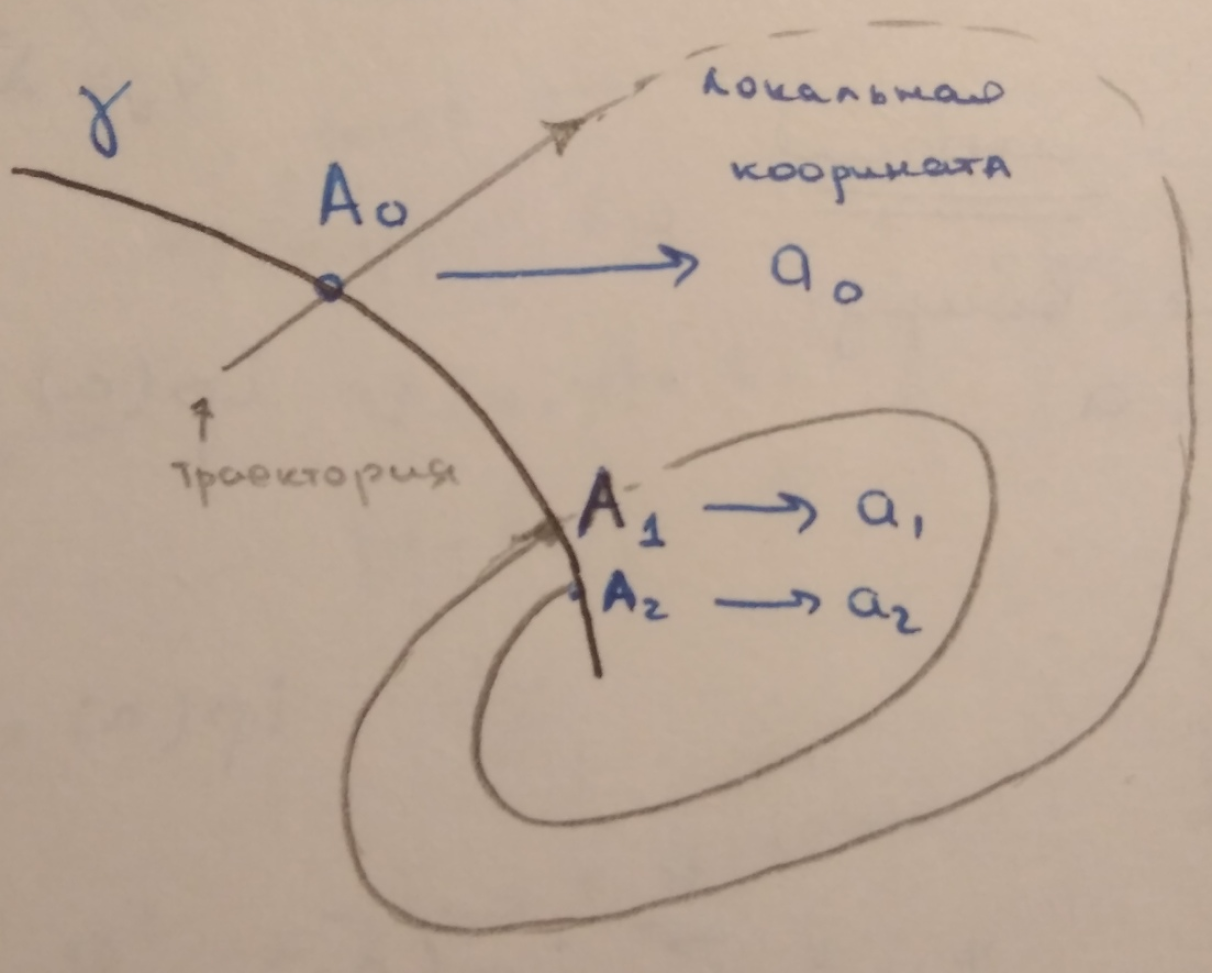
\includegraphics[width=0.7\textwidth]{ch8/pict/pict_1.png} \end{center} 
				\begin{center}2 варианта: \end{center}  
				1) траектория ушла \newline
				2) траектория вернется. Тогда по непрерывности, \newline 
					после $A_1$ она попадет еще и в $A_2$.
	\end{minipage} \newline
	\begin{assertion}{\label{afKul}}
		Чтобы через $A_0$ проходила замкнутая траектория ($\psi$ определена в окрестности $A_0$)
			необходимо и достаточно, чтобы $\psi(a_0)=a_0$ или П$(a_0) = 0$
	\end{assertion}
	\begin{proof} Необходимость  очевидна \newline
	
		Достаточность: Докажем от противного. Пусть $a_1 =\psi(a_0) \neq a_0$ \newline
		\begin{minipage}{0.35\textwidth} 
			\vspace{3mm}
			\begin{center} 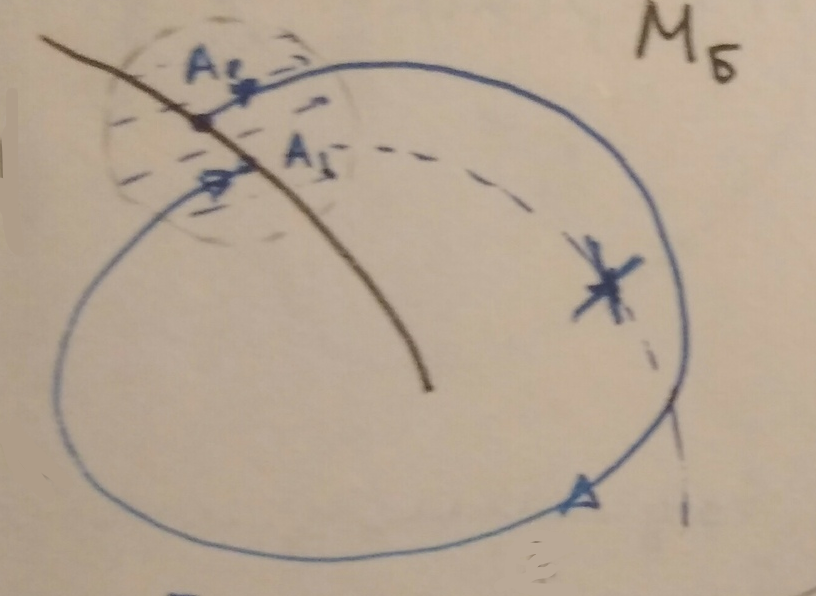
\includegraphics[width=0.9\textwidth]{ch8/pict/pict_2_1.png} \end{center} 
			$$M_\text{Б}\text{ --- мешок Бендиксона}$$
			Мы его не можем пересекать $\Rightarrow$ \newline 
			\hspace*{15mm} не вернемся в $a_0$.
		\end{minipage}
			\hfill
		\begin{minipage}{0.32\textwidth}
			\begin{center} 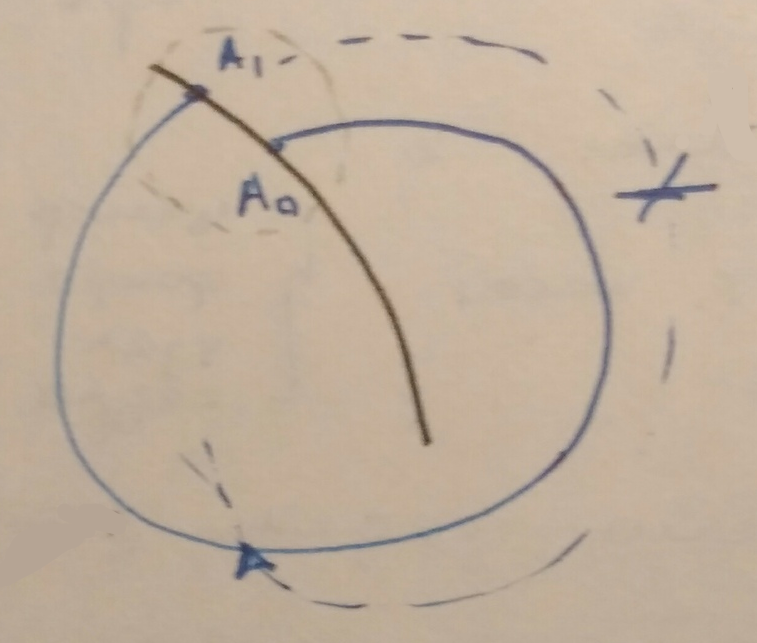
\includegraphics[width=1\textwidth]{ch8/pict/pict_2_2.png} \end{center} 
				\qquad \qquad  Аналогично, \newline \hspace*{13mm} но вне мешка. \newline
		\end{minipage}
		\begin{minipage}{0.31\textwidth}
			\begin{center} 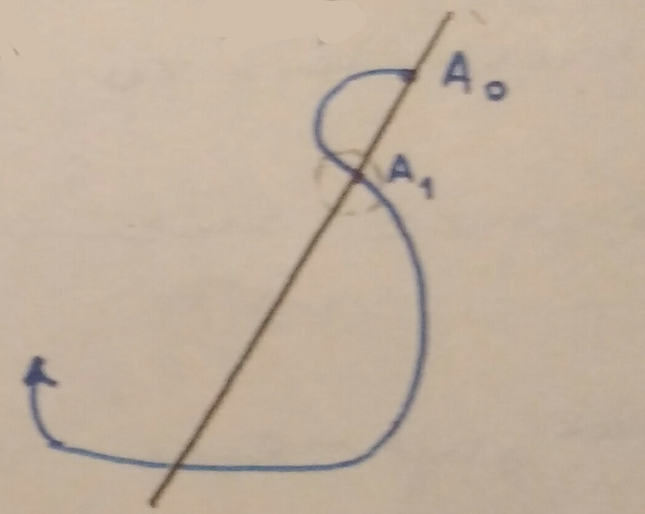
\includegraphics[width=1\textwidth]{ch8/pict/pict_2_3.png} 
				Направление поля  \newline поменялось, такого \newline не может быть. \end{center} 
		\end{minipage}		
		
	\end{proof}

 	\newpage
	\begin{minipage}{0.1\textwidth} 
		$$
			\begin{cases}
	 			\dot{x} = f_1(x,y) \\
	 			\dot{y} = f_2(x,y)
			\end{cases} 
		$$
		$$
			\begin{gathered}
				a_1 = \psi(a_0) \\
				a_2 = \psi(a_1)  \\ \cdots \\
				a_k =\psi(a_{k-1}) 	\\ \cdots		
			\end{gathered}
		$$
	\end{minipage}
		\hfill
	\begin{minipage}{0.5\textwidth}
		\cntrKul Имеет отображение $\psi: a_{k+1} = \psi(a_k)$ \cntrKul \newline
		\cntrKul Если есть $a^*: \psi(a^*)=a^* \Rightarrow$ траект. замкнута \cntrKul \newline 
		\cntrKul Точка $a^*$ устойчивая, если $|\psi'(a^*)|<1$	\cntrKul \newline 
		\cntrKul Точка $a^*$ неустойчивая, если $|\psi'(a^*)|> 1$ \cntrKul
		\begin{center} 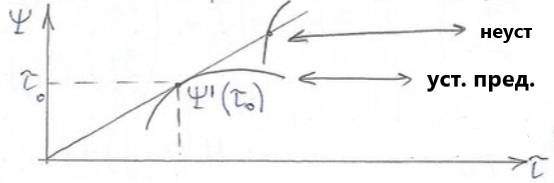
\includegraphics[width=0.7\textwidth]{ch8/pict/pict_3_2.png} \end{center} 
	\end{minipage}
	\begin{minipage}{0.31\textwidth}
		\begin{center} 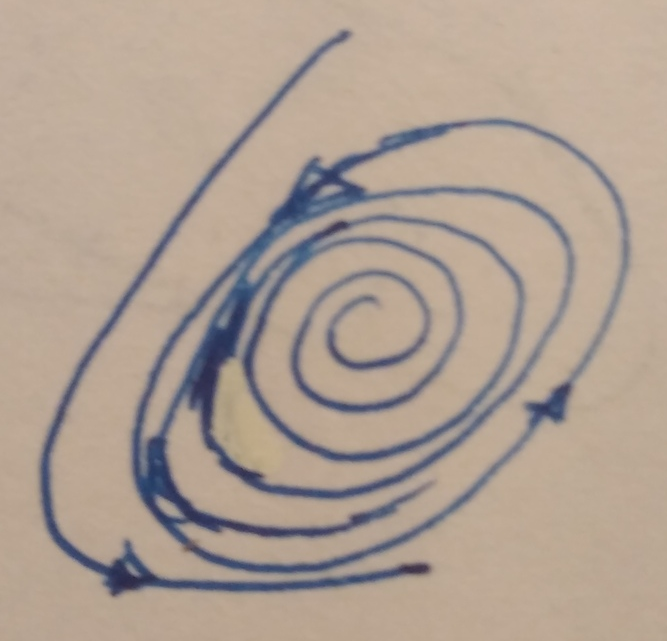
\includegraphics[width=0.8\textwidth]{ch8/pict/pict_3_1.png} \end{center} 
		\cntrKul Если точка $a^*$ устойчивая, \cntrKul \newline
		\cntrKul то есть устойчивый  \cntrKul \newline
		 \cntrKul предельный цикл  \cntrKul
	\end{minipage}		
	
	То же самое можно определить и в пространстве: \vspace{7mm}
	
	\begin{minipage}{0.4\textwidth}
		\begin{center} 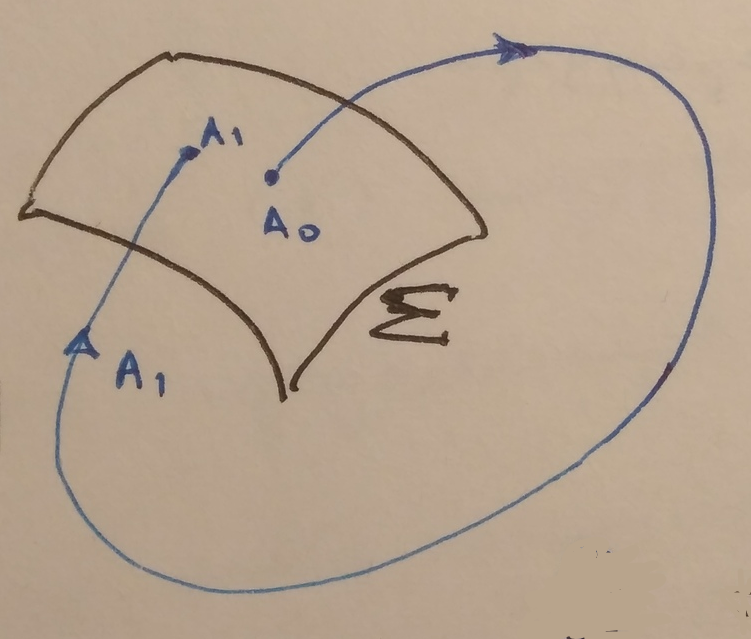
\includegraphics[width=1\textwidth]{ch8/pict/pict_4.png} \end{center} 
	\end{minipage}
	\begin{minipage}{0.58\textwidth}
		\cntrKul Предыдущее утв. $\ref{afKul}$ не верно в $\mathbb{R}^m$, но: \cntrKul \newline
		$$\begin{gathered}
			A_0(a^0) \rightarrow A_1(a^1), \quad a^k=(a^k_1,\cdots,a^k_m) \vspace{2mm}\\
			a^{k+1} = \Psi(a^k), \quad \Psi = (\Psi_1, \cdots, \Psi_m) \\
			\text{Матр. Якоби: }	 \left( \dfrac{\partial\Psi}{\partial a} \right) = 	 
					 \begin{pmatrix} \frac{\partial\Psi_1}{\partial a_1} & \cdots & \frac{\partial\Psi_1}{\partial a_m} \\
					 						  \cdots & \cdots & \cdots & \\
					 						   \frac{\partial\Psi_m}{\partial a_1} & \cdots & \frac{\partial\Psi_m}{\partial a_m}
					  \end{pmatrix}	
		\end{gathered}$$ 
		 \cntrKul Мультипликатор $\mu$ --- соб. зн. матрицы Якоби\cntrKul \newline
		 \cntrKul Усл. уст. особой точки: $|\mu_i|<1, \quad i=\overline{1,m}$\cntrKul 
	\end{minipage}		
	\newline 
	
	\begin{theorem}
		Система Лотки-Вольтерры не имеет предельных циклов
		\begin{equation}
			\begin{gathered}
				\dot{x} = x(r_1+a_{11}x+a_{12}y) \\
				\dot{y} = y(r_2+a_{21}x+a_{22}y)
			\end{gathered}	\label{ch10_LVS}
		\end{equation}
	\end{theorem}
	\begin{lemma}
			Пусть задана система ($\ref{ch10_LVS}$), а $V(x,y)$ --- интеграл системы, 
			т.е. \newline $V(x,y) \equiv const$, то такая система не имеет предельных циклов. 
	\end{lemma} 
	\begin{proof}{ Начнем с леммы:} \vspace{3mm}
	
		\begin{minipage}{0.3\textwidth}
			\begin{center} 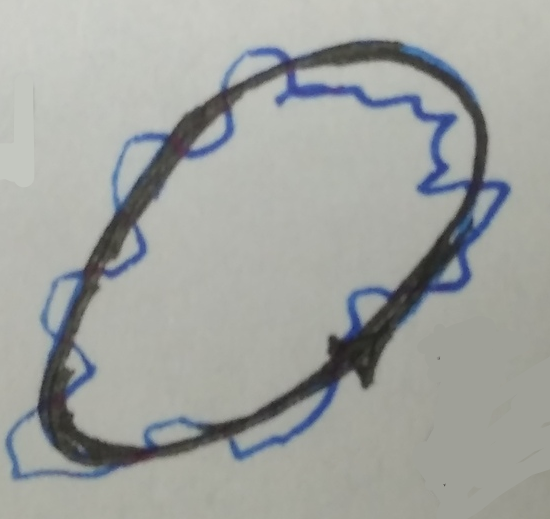
\includegraphics[width=0.5\textwidth]{ch8/pict/pict_5.png} \end{center} 
		\end{minipage}
		\begin{minipage}{0.58\textwidth}
			$$\left.
				\begin{gathered}
					V(x,y) = c_0 \\
					V(x,y) = \tilde{c_0} \\
					|c-\tilde{c_0}| < \varepsilon
				\end{gathered} \quad \right|\Rightarrow \quad 
			$$ пришли к противоречию с тем, что вблизи предельного цикла нет других замкнутых траекторий
		\end{minipage}		
		
	\end{proof}
	\begin{proof}{ Теперь докажем саму теорему} \vspace{3mm}
	
		Пусть $\exists \gamma \in \mathbb{R}^2_+ \Rightarrow$ по т. Пуанкаре $\exists a$ --- неподвижная точка 
		в $\gamma$ 
		\newline
		
		\begin{minipage}{0.3\textwidth}
			\begin{center} 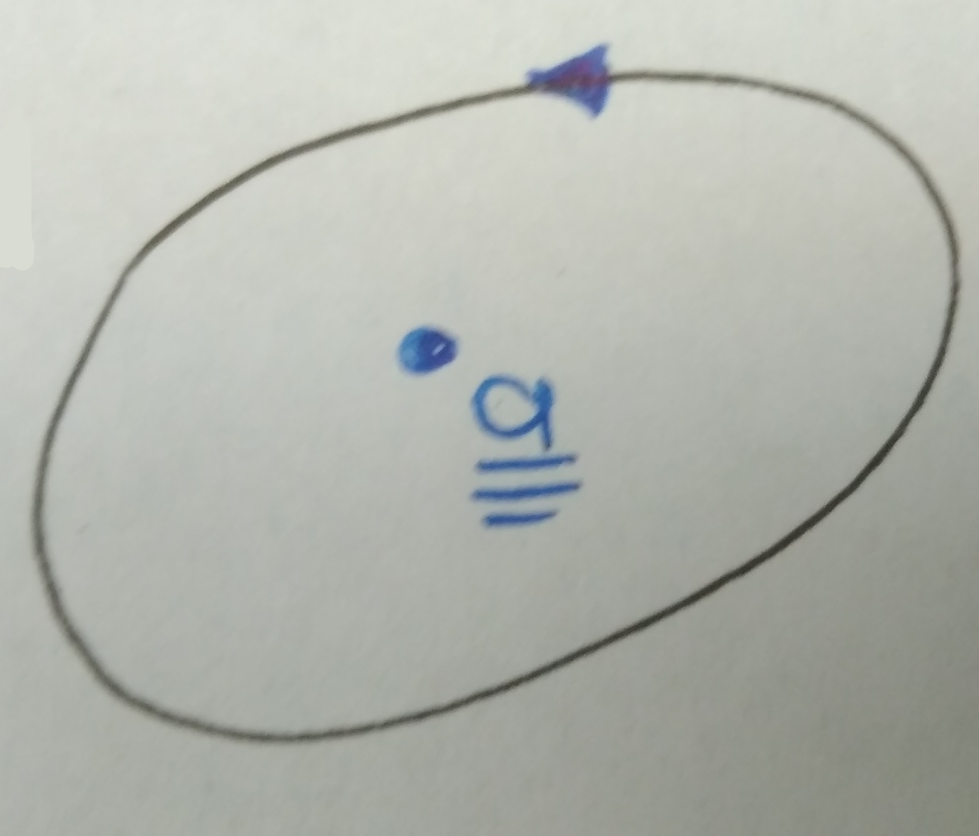
\includegraphics[width=0.7\textwidth]{ch8/pict/pict_6.png} \vspace{3mm}\end{center} 
		\end{minipage}
		\begin{minipage}{0.68\textwidth}
			$$
				\begin{gathered}
					a_{11}x + a_{12}y = -r_1 \\
					a_{21}x + a_{22}y = -r_1 \\
				\end{gathered} \qquad  \Delta = a_{11}a_{22} - a_{12}a_{21} \neq 0
			$$ \cntrKul Введем $\mu = x^{\alpha-1}y^{\beta -1}>0, \quad \alpha, \beta \in \mathbb{R}^2_+$ \cntrKul
			\begin{equation}
				\begin{gathered}
						\dot{x} = y^{\beta -1} x^{\alpha}(r_1 + a_{11}x + a_{12}y) \\
						\dot{y} = y^{\beta} x^{\alpha-1}(r_2 + a_{21}x + a_{22}y) 
				\end{gathered}\label{ch10_orb_eq} \qquad 
		\end{equation}
		\end{minipage}		
		
		Системы ($\ref{ch10_LVS}$) и ($\ref{ch10_orb_eq}$) топологически орбитально эквивалентны. 
		$$
		\begin{gathered}
			\textrm{div} f = y^{\beta-1} x^{\alpha-1}\alpha(r_1 + a_{11}x + a_{12}y) + 
										y^{\beta -1} x^{\alpha}a_{11} +
										\beta y^{\beta -1} x^{\alpha-1}(r_2 + a_{21}x + a_{22}y) + 
										y^{\beta} x^{\alpha-1} a_{22} = \\
			= y^{\beta-1} x^{\alpha-1} (\alpha (r_1 + a_{11}x + a_{12}y) 
							+ x a_{11} +\beta (r_2 + a_{21}x + a_{22}y) + y a_{22}) = \\
			= y^{\beta-1} x^{\alpha-1} \left\{ [\alpha a_{11}+ a_{11}+\beta a_{11} ]x +
								[\alpha a_{12} + \beta a_{22} + a_{22}]y + \alpha r_1+ \beta r_2 \right\}
		\end{gathered}
		$$
		Мы утверждаем, что для $\quad \begin{cases}
													\alpha a_{11} + \beta a_{21} = -a_{11} \\
													\alpha a_{21} + \beta a_{22} = -a_{22}
												\end{cases} \quad \exists(\alpha^*, \beta^*): \Delta \neq 0 \Rightarrow \quad
												\vspace{2mm}$\newline
												
		\textrm{div} $\mu f = x^{\alpha-1}y^{\beta -1}(\alpha^* r_1 + \beta^* r_2) $. Варианты:
		\begin{enumerate}
			\item $\alpha^* r_1 + \beta^* r_2 \neq 0 \Rightarrow$ знакоопр. и воспользуемся т. Дюлака-Бендиксона.
			\item $\alpha^* r_1 + \beta^* r_2 \neq 0 \Rightarrow$ существует первый интеграл $\Rightarrow$
					замкнутая траектория \newline не может быть изолированной. Покажем это:
					$$
						\iint\limits_{D_\gamma}\left( \dfrac{\partial F_1}{\partial x} + 
																		\dfrac{\partial F_2}{\partial y} \right)dx\,dy = 
						\int\limits_{\gamma} F_2 dx + F_1 dy = 0, \qquad 
						\begin{gathered}
							F_1 = Q(x,y)\\
							F_2 = -P(x,y)
						\end{gathered}
					$$
					$$
						\begin{gathered}
						\exists \Phi(x,y): d\Phi(x,y) = Pdx+Qdy \Rightarrow d\Phi(x,y) = -F_2dx+F_1dy \Leftrightarrow \\
							 \Leftrightarrow \Phi(x,y) \equiv \textrm{const} \text{ и это первый интеграл.}
						\end{gathered}
					$$
		\end{enumerate}
	\end{proof}

	\begin{theorem} \textbf{Теорема Бендиксона-Пуанкаре \vspace{5mm}} \newline
			\begin{equation}
				\begin{gathered}
						\dot{x} = f_1(x,y) \\
						\dot{y} =f_2(x,y)
				\end{gathered} \quad \bar{D} \subset \mathbb{R}^2 \ \label{ch10_bend_puanc} \qquad 
			\end{equation}
			Условия:
			\begin{enumerate}
				\item $\bar{D}$ --- огр. замкн. обл. в $\mathbb{R}^2$
				\item $\bar{D}$ --- положительно инвариантно относительно системы $(\ref{ch10_bend_puanc})$ :
					$$
						(x_0, y_0) \in \bar{D}, \quad \left. \begin{gathered}
																				x = x(x_0,y_0) \\
																				y = y(x_0,y_0)
																			\end{gathered} \right\} \quad \gamma \subset \bar{D}
					$$
				\item $\bar{D}$ не содержит неподвижных точек системы $(\ref{ch10_bend_puanc})$.
			\end{enumerate}
			Тогда в $D$ $\exists$ по крайней мере одна замкнутая траектория. 	
	\end{theorem}
	
	\begin{minipage}{0.6\textwidth}
		\begin{lemma}
			Если траектории системы $(\ref{ch10_bend_puanc})$ содержат хотя бы одну свою предельную точку
			при $t\rightarrow\infty$, то это либо точка покоя, либо цикл.
		\end{lemma} 
	\end{minipage}
	\hfill
	\begin{minipage}{0.3\textwidth}
		\begin{center} 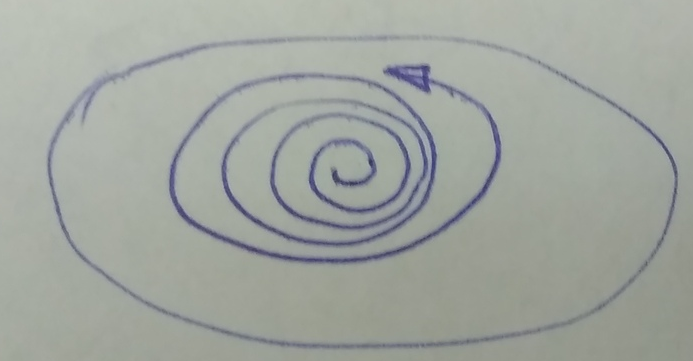
\includegraphics[width=0.8\textwidth]{ch8/pict/pict_8.png} \vspace{5mm}\end{center} 
	\end{minipage}

	\begin{proof}
		\begin{itemize}
			\item Пред. точка --- очевидно. 
			\item Иначе, в окр. точки по теореме о выпрямлении векторного поля получим:
		
			\begin{minipage}{0.4\textwidth}
				\cntrKul $(\bar{x}, \bar{y})$ --- не точка покоя \cntrKul \newline
				Пусть траектория не замкнута. \newline 
				Тогда по т. о непрерывной зависимости решения имеем 2 случая,
				 	показанных на рисунках. Применим к обоим из них мешок Бендиксона и получим противоречие.
			\end{minipage}
				\hfill
			\begin{minipage}{0.24\textwidth}  \vspace{3mm}
			
				\begin{center} 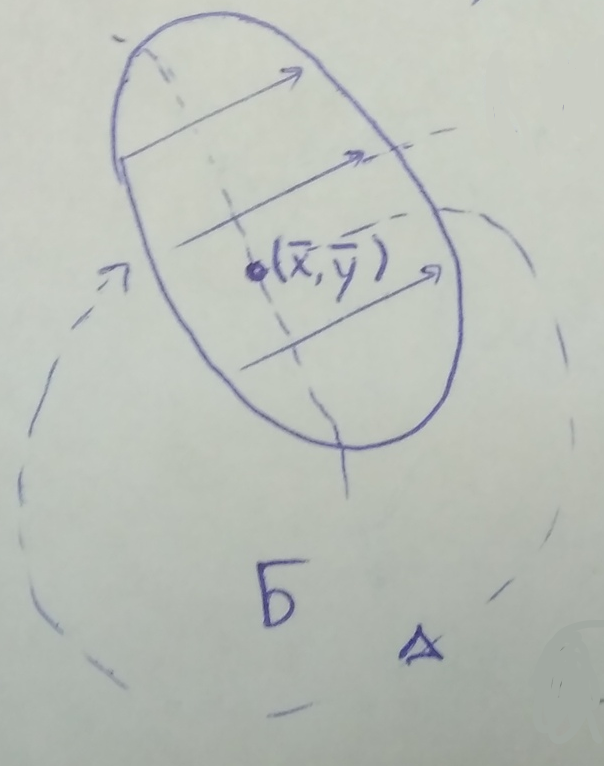
\includegraphics[width=0.9\textwidth]{ch8/pict/pict_9_1.png}\end{center} 
			\end{minipage}
			\begin{minipage}{0.24\textwidth} \vspace{4mm}
			
				\begin{center} 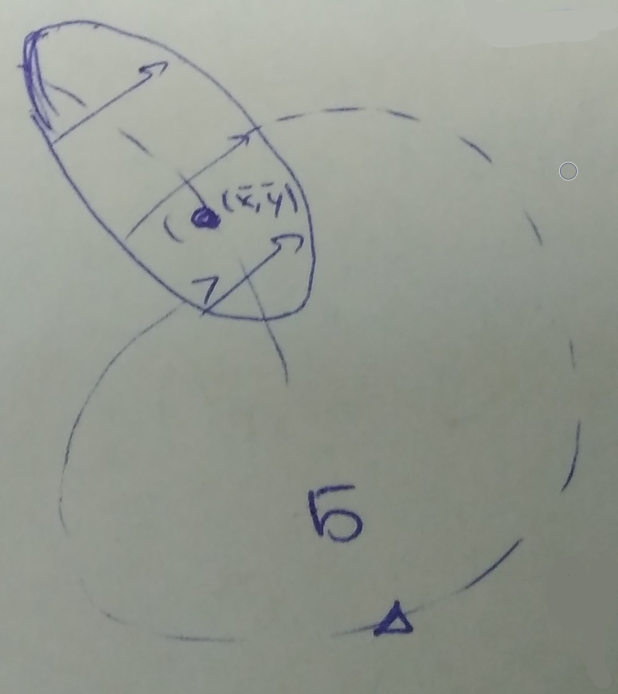
\includegraphics[width=0.95\textwidth]{ch8/pict/pict_9_2.png} \vspace{5mm}\end{center} 
			\end{minipage}
				
		\end{itemize}		
		
	\end{proof}
	\noindent
	\begin{lemma}
		Пусть траектория системы $\gamma$ при $t\rightarrow \infty$ имеет предельную точку $\bar{M}\in\gamma$, 
		принадлежащую некоторой замкнутой кривой. Тогда либо $\gamma = \bar{\gamma}$, либо $\gamma$ 
		спиралевидно приближается к $\bar{gamma}.$
	\end{lemma}
	\begin{proof}
		\begin{itemize}
			\item Траектория $\gamma$ проходит через $\bar{M}\in\bar{\gamma}\Rightarrow x(t,\bar{M})	
																															\in\bar{\gamma}$
			\item Траектория проходит близко от $\bar{M}$
			\newline
			\begin{minipage}{0.3\textwidth}  \vspace{3mm}
				\begin{center} 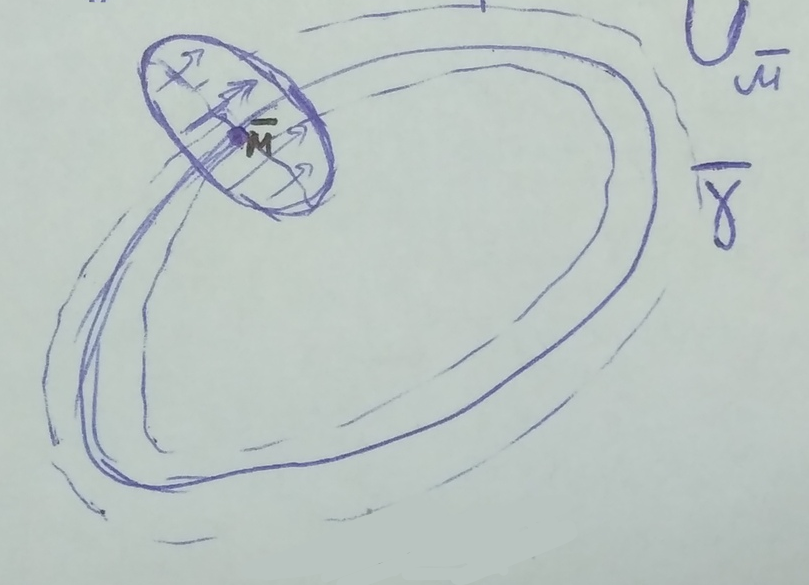
\includegraphics[width=0.9\textwidth]{ch8/pict/pict_10.png}\end{center} 
			\end{minipage}
				\hfill
			\begin{minipage}{0.6\textwidth} \vspace{4mm}
				\cntrKul $\bar{M}$ --- предельная $\Rightarrow \, \exists a \in U_{\bar{M}}$ \cntrKul \newline
				$\rho(a, \bar{M}) > \rho(b, \bar{M}) > \ldots $ (иначе $\bar{M}$ --- не предельная).
			\end{minipage}
				
		\end{itemize}
	\end{proof}
	\begin{proof}{ Докажем теорему Бендиксона-Пуанкаре} \vspace{3mm}
	
		Из точки выпустим траекторию $ \gamma: \left\{ \begin{gathered}
																				x = x(t, x_0) \\
																				y = y(t,y_0)
																			\end{gathered} \quad \right. (x_0, y_0) \in \bar{D}.
															$ Она не покидает $\bar{D}$.\vspace{3mm} \newline
		По т. Вейерштрасса можно выделить $\{t_k\}$ сходящуюся 
																			$\quad \begin{gathered}
																				x_k = x(t_k,x_0) \\
																				y_k = y(t_k,y_0)
																			\end{gathered} \,\, \rightarrow 
																			\begin{pmatrix} \bar{x}\\ \bar{y} \end{pmatrix} = \bar{M}
																			$ \newline
		2 варианта:
		\begin{itemize}
			\item $\bar{M} \in \gamma \Rightarrow$ по первой сопутствующей доказательству лемме получим, что 
				$\gamma$ --- замкнутая траектория.
			\item  $\bar{M} \notin \gamma$ \newline
					$ \left. \begin{gathered}
										x = x(t, x_0) \\
										y = y(t,y_0)
									\end{gathered} \quad \right\} \bar{\gamma} \quad								 
								\{t_n\} \quad
								\begin{gathered}
									x_n = x(t_n,\bar{x}) \\
									y_n = y(t_n,\bar{y})
								\end{gathered} \,\, \rightarrow 
								\begin{pmatrix} \bar{\bar{x}}\\ \bar{\bar{y}} \end{pmatrix} = \bar{\bar{M}}
								$ \newline
				Из инвариантности предельного множества $\Rightarrow$ $\bar{\gamma}$ --- предельная 
					$\Rightarrow$ опять 2 варианта:
						\begin{itemize}
								\item $\bar{\bar{M}}\in \bar{\gamma} \Rightarrow$ $\bar{\gamma}$ --- замкнутая траектория.
								\item  $\bar{\bar{M}} \notin \bar{\gamma}$, $\tilde{a}\in \bar{\gamma}$. 
								$\bar{\bar{M}}$ --- пред. и $\tilde{a}$ --- предельная, противоречие.						
						\end{itemize}
						\begin{center}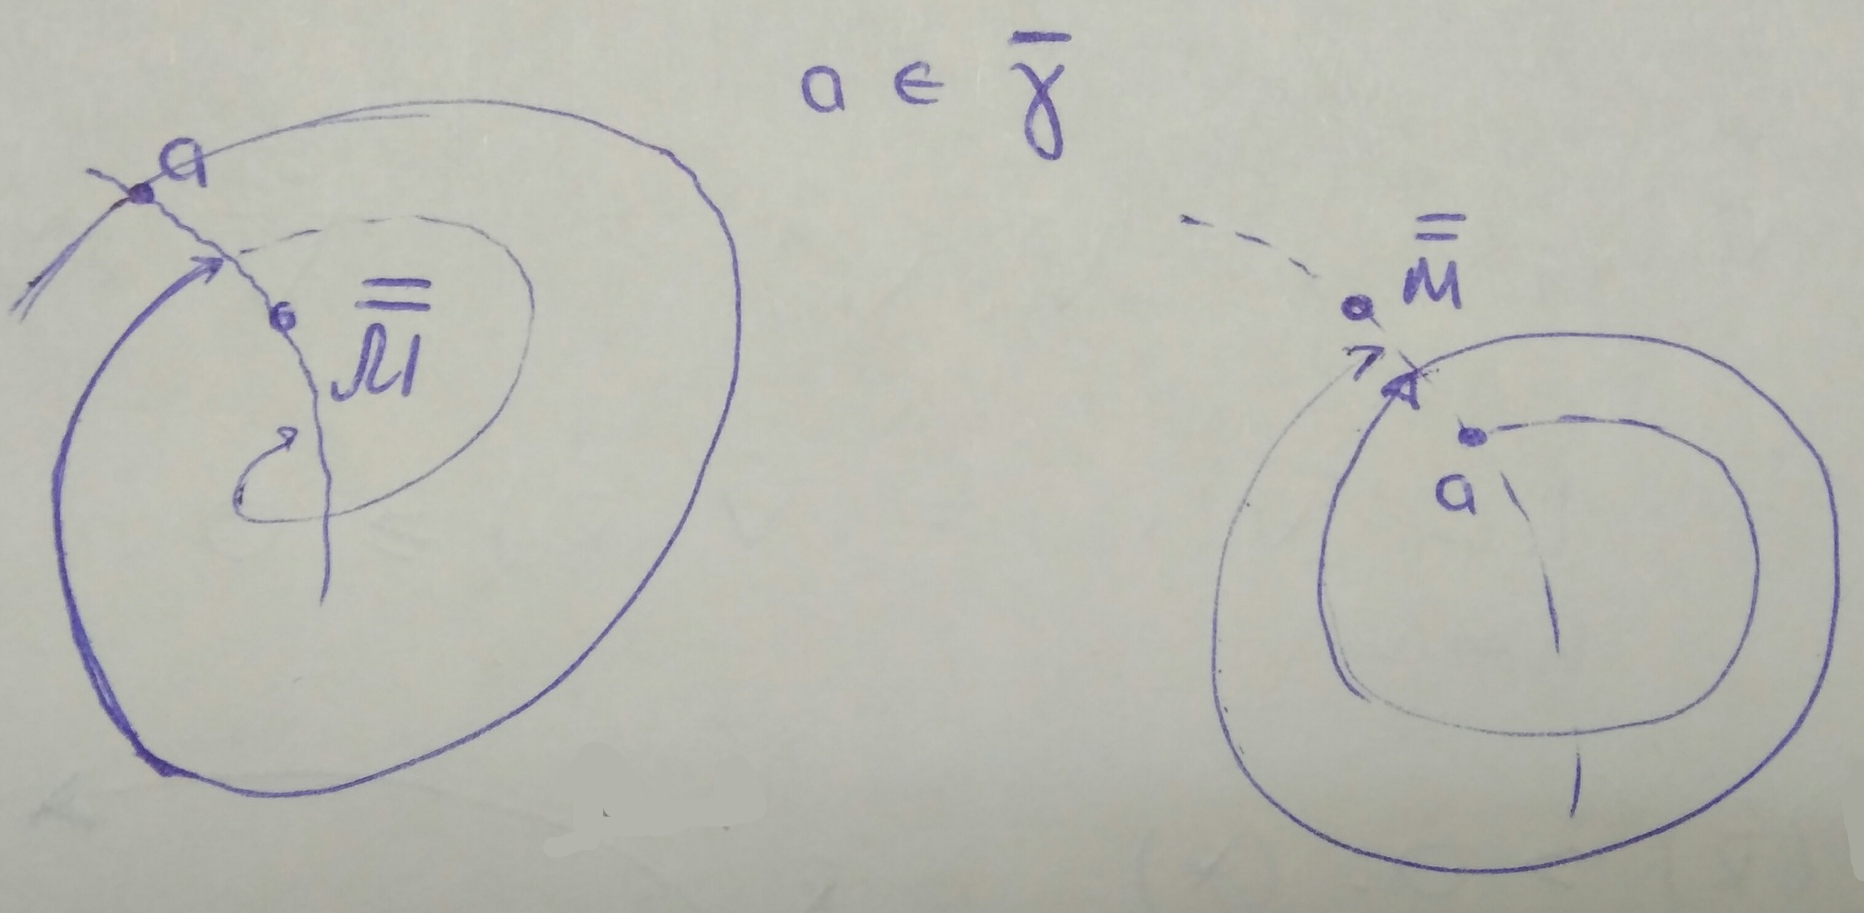
\includegraphics[width=0.55\textwidth]{ch8/pict/pict_11.png}\vspace{5mm}\end{center} 
		\end{itemize}
	
	\end{proof}

	\begin{minipage}{0.4\textwidth}
		
		\begin{example}
		$$
			\begin{cases}
				\dot{x} = y \\
				\dot{y} =-x
			\end{cases} \Rightarrow  \quad  \begin{gathered} x^2+y^2 = R^2, \\ \text{нет пред. цикла,}\\ \text{хоть
									 и выполнены условия} \end{gathered} 
		$$
		\end{example}
	\end{minipage} 
		\hfill
	\begin{minipage}{0.4\textwidth}	
		\begin{center} 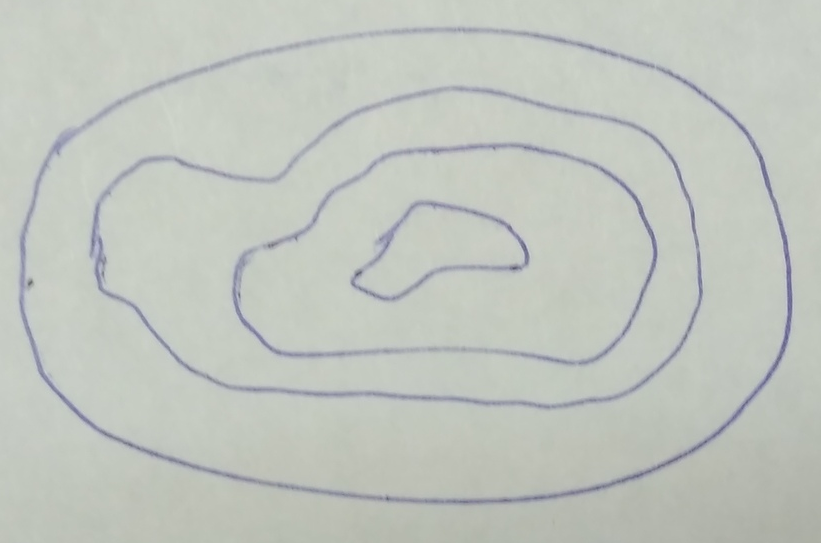
\includegraphics[width=0.6\textwidth]{ch8/pict/pict_7.png} \vspace{5mm}\end{center} 
	\end{minipage} 	
	
	\begin{assertion} (Следствие)
	 	
			Пусть в некоторой окр. $\bar{\gamma}$ нет других замкнутых траекторий. Тогда все траектории,
			 начинающиеся вблизи $\bar{\gamma}$, спиралевидно стремятся к $\bar{\gamma}$.
	\end{assertion}

	\begin{theorem} \textbf{Теорема Брауэра}
	
		Пусть $K \subset \mathbb{R}^n$ и $K$ --- голоморфно ($\exists$  гладкое взаимноодн. отображение) 
			шару. \newline Пусть есть $\psi: K\rightarrow K$. Тогда:
		$$	
			\exists x^0: \psi(x^0) = x^0, \quad x^0\in K
		$$
	\end{theorem}
	\begin{theorem} \textbf{Теорема Ла-Cалля} (о монотонности функции Ляпунова)
	
		$$
			\dot{x} = f(x) \qquad x \in D \in \mathbb{R}^n
		$$\newline
		Пусть $V(x)$ --- некоторая функция: $\quad \begin{gathered}
																			1) V(x) \in \mathbb{C}^1(D) \\
																			2) \dot{V}(x) \geqslant 0 \, (\leqslant 0)
																		\end{gathered}\vspace{3mm}$ \newline
		Рассмотрим множества $\alpha= \left\{x \in D\Big| \dot{V}(x) = 0\right\}$ и $W_{lim}$ --- мн-во всех пред. 
																				точек в $\bar{D}.$ Тогда: 
				$$
					 [W_{lim}\cap D] \subset \alpha
				$$
	\end{theorem}
	\begin{proof} \newline
		Пусть $\bar{x} \in W_{lim}\quad \exists t_k: \, x(t_k,x^0) \rightarrow \bar{x}$;
		$\dot{V}(x) \geqslant 0 , \dot{V}(x(t_k, x^0))\geqslant 0 \quad \lim\limits_{t_k\rightarrow \infty}
																\dot{V}(x(t_k, x^0)) = \dot{V}(\bar{x}) $ \newline
		Если $\dot{V}(x) = 0$, то доказано. \newline
		Предположим, что $\dot{V}(x) > 0$\newline
		\begin{minipage}{0.4\textwidth} \vspace{3mm}		
			\begin{center} 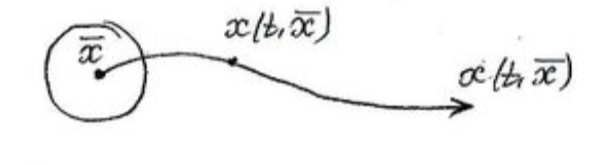
\includegraphics[width=0.6\textwidth]{ch8/pict/pict_13_1.png} \vspace{5mm}\end{center} 
		\end{minipage} 
		\begin{minipage}{0.4\textwidth}	
			$$V(x(t,\bar{x})) > V(\bar{x})\quad (*)$$
		\end{minipage} 	
		\newline
		\begin{minipage}{0.4\textwidth} \vspace{3mm}		
			\begin{center} 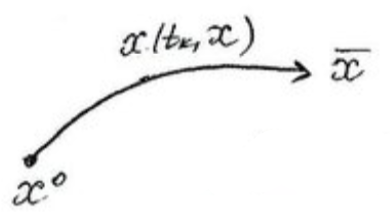
\includegraphics[width=0.6\textwidth]{ch8/pict/pict_13_2.png} \vspace{5mm}\end{center} 
		\end{minipage} 
		\begin{minipage}{0.4\textwidth}	
			$$\begin{gathered}  x(t_k,x^0) \rightarrow \bar{x}, \quad \dot{V}(x)\geqslant 0 \\
												 V(x(t_k, x^0)) \leqslant V(\bar{x}) \end{gathered}$$
		\end{minipage} \newline	
		$x(t+t_k,x^0)$ = \{ групповое св-во \} = $x(t, x(t_k,x^0)), \quad 
										\lim\limits_{t_k\rightarrow \infty} x(t,x(t_k,x^0)) = x(t,\bar{x})$
		$$
			V(x(t_k+t,x^0)) \leqslant V(\bar{x}) \Rightarrow V(x(t,\bar{x})) \leqslant V(\bar{x}) \quad (**)
		$$
		Пришли к противоречию с предположением, что $\dot{V}(\bar{x})>0$.
		
	\end{proof}
	
	
	\begin{example}Использование теоремы Ла-Салля
		$$			
			\begin{cases}
				\dot{u} = u(1- v -\alpha u) \\
				\dot{v} = v(-\gamma + u -\beta v) 
			\end{cases} \qquad \begin{gathered} (u,v) \in \mathbb{R}^2_+ \\ \alpha, \beta, \gamma > 0\end{gathered}
		$$
		$$
			\begin{cases}
				 \alpha u^* + v^* =1 \\
				 u^* - \beta v^* = \gamma 
			\end{cases} \qquad  (u^*,v^*) \in \mathbb{R}^2_+ \qquad V = (u^*\ln u- u )x + (v^*\ln v - v) y
		$$
		$$
			\begin{gathered}
				\dot{V} = \dfrac{\partial V}{\partial u} \dot{u} + \dfrac{\partial V}{\partial v} \dot{v} = 
					\left( \dfrac{u^*}{v} -1 \right) u \left(1-v-\alpha u\right)x + 
					\left( \dfrac{v^*}{v} -1 \right) v \left(-\gamma+u-\beta v \right)y = \vspace{2mm} \\
					= (u^* -v^*)(\alpha u^* + v^* -v -\alpha u)x + (v^*-v)(\beta v^* - u^* +u-\beta v)y =
																															 \{x=y=1\} =  \vspace{2mm} \\
					= \alpha(u^*-u)^2+ \beta(v^*-v)^2
			\end{gathered}
		$$	
		$$
			\dot{V} \geqslant 0 \qquad \dot{V}(u^*,v^*) = 0 \quad \Rightarrow \quad W_{lim} = 
						\begin{cases}
							u =u^* \\
							v = v^*
						\end{cases} \leftarrow \quad \begin{gathered} \text{глобально} \\
																					 	\text{уст. точка} \\
																						  \text{равновесия}	 
															\end{gathered}
 		$$
	\end{example}

